% vim: set fenc=utf-8 ft=latex encoding=utf-8
% -*- mode: latex; coding: UTF-8; -*-
%!TEX root = knowledge-curation.tex

\section{Discussion}
\label{cha:theory}

In this section, we reflect on the results presented in the previous section and place them within the context of related research. Additionally, we identify research opportunities and derive recommendations for using multiple Q\&A channels.
In the following, we provide representative quotes extracted from the survey, using P\# to indicate the participant ID.

\subsection{Knowledge Creation and Curation}

    Based on the results, both channels seem to provide roughly the same knowledge support for questions and answers.
    However, there are some important differences between the channels, which are summarized in Table~\ref{table:constrat}. We discuss each in detail below.
%    These observations are tendencies, and they are not behaviours unique of each channel.

    \begin{table}[!htb]
      \centering
      \caption{Comparison of the way knowledge is shared on \SO and the \RH mailing list.}
      \label{table:constrat}
      \begin{small}
        \setlength{\tabcolsep}{5pt}
        \begin{tabular}{@{}lll@{}}
          \toprule
          \textbf{}      & \textbf{\SO} & \textbf{\RH}\\
          \midrule
          Knowledge construction & Mainly crowd             & Mainly participatory \\
          Topic restriction      & Yes & No \\
          Emphasis & Curating knowledge & Developing knowledge \\ 
          \bottomrule
        \end{tabular}
      \end{small}
\vspace{-3mm}
    \end{table}

\subsubsection{Knowledge construction}

\SO's gamification mechanism encourages users to be first when answering questions~\cite{Singer2013}. In contrast, the \RH mailing list is a less competitive
environment, where users tend to build on other responses. In \RH, users work as a team, rather than as individuals searching for points (as is the case on \SO).
As a result, knowledge on \SO is built in a more crowdsourced manner, while knowledge on the \RH mailing list is usually built in a participatory manner.

The competitive \SO environment creates an incentive to be the first to answer, rather than improving and building on other answers. It's not uncommon to find a question with several answers that provide the same information. For example, three of the six answers in the \SO question titled \textit{``Resources for learning SAS if you are already familiar with R''}\footnote{\url{http://goo.gl/Mb4Pbk}} referenced the same books.
%    The gamification mechanism gives reputation to those who answer the questions, even when each extra answer might not add any new insight about how to solve a specific problem.
And while \SO provides a powerful curation mechanism to ensure the best answers make it to the top, it does not explain why an answer is better than another.

In contrast, the \RH mailing list tends to be more participatory in how users construct knowledge and it fosters an environment where users discuss proposed answers. Its users tend to provide more background to the answers and explain the rationale behind them.

For example, the question \textit{``Arrange elements on a matrix according to rowSums + short `apply' Q''} was posted to both \SO\footnote{\url{http://goo.gl/a8AES8}} and {\RH}\footnote{\url{http://goo.gl/PGflT5}}. This question illustrates the contrast in how the two communities build knowledge.
On \SO, each participant contributed a solution without any evidence of collaboration with others.
Whereas users on the \RH mailing list complemented each other's answers by providing further information and insights to the answers already
contributed. Vasilescu \textit{et al.}~\cite{Vasilescu2014c} showed that members who are active in both channels tend to provide answers faster on \SO than on \RH,
suggesting that they are motivated by the gamification aspects of \SO, and thus they tend to gravitate towards crowd knowledge construction.

    
While prevalent, the construction of knowledge on \SO is not limited to the crowd-based approach. Participatory knowledge construction is also existent, such as by up/down voting questions and providing comments. In most cases, participatory knowledge construction on \SO is used for editing answers (e.g., correcting grammar) or linking to previously asked questions.
Similarly, some knowledge on the \RH mailing list is constructed in a crowd-based manner, but this form is less prevalent than the participatory one.

Tausczik \textit{et al}.~\cite{Tausczik2014} examined how members of Math Overflow (a Q\&A platform for mathematicians) collaborate and construct knowledge. They found that collaboration was diverse and fell on the spectrum between \textit{independent} (crowd-based) and \textit{interdependent} (participatory). Similar to our findings with \SO, the most common collaborative act was of an independent nature (i.e., providing information), while other contributions that built on existing work were less common (i.e., clarifying the question, critiquing answers, revising answers, and extending answers).

Our results seem to imply that \SO's gamification features, while highly effective, have the side effect of reducing collaborative knowledge creation between users. In their study on building \SO reputation, Bosu \textit{et al.}~\cite{Bosu2013} proposed six strategies for increasing reputation score, two of which were: be the first to answer, and do it at \textit{off-peak hours}---indicating crowd knowledge creation. Furthermore, while \SO gives people the ability to vote on comments, it does not reward points to users that post comments. For example, some users search \SO for answers within comments and convert them to proper answers to gain reputation points\footnote{\url{http://duncanlock.net/blog/2013/06/14/the-smart-guide-to-stack-overflow-zero-to-hero}}.


    % The findings presented here as theory can be used to identify how channels' features or community members might affect the construction of knowledge.
    % For instance, we identified that gamification might affect collaboration between users. 
    % Users prefer to create their own answer instead of collaborating with others.
    % Additionally, it might be possible for indirect collaboration, like the one happening on the comments on \SO to improve discussion and participatory knowledge construction if there was a mechanism to provide points for this type of participation.
%    However, more studies are required to extend our observation to other domains, communities, and channels.

\subsubsection{Topic restriction}

\SO's participation rules only permit questions that have a clear answer, making it topic restrictive. In contrast, the \RH mailing list is suitable for discussing
any topic related to the R language. For example, questions related to R but not focused on software development are not rejected by the \RH mailing list community---topics that trigger discussion are welcomed!
%    For instance, when users discuss the creation or improvement of the R community channels (see section \ref{sec:userbeh}); or when a question about installing R on \textit{Linux} is asked on the \RH mailing list (like {\href{http://goo.gl/1JLOUF}{\textit{``R on X11 under Linux''}}}).

\SO questions that trigger a discussion are flagged as opinion-based or off-topic and will likely be closed. Correa and Sureka~\cite{Correa2014} found that 18\% of deleted questions on \SO are subjective (i.e., ask for opinion).
For example, a question titled \textit{``What's a good example of really clean and clear [R] code, for pedagogical purposes?''}\footnote{http://goo.gl/9JjZW1} was flagged as \textit{off-topic} because the question was not related to software development.
An \RH user wrote a fine explanation of the purpose of each channel in a message on the mailing list:\footnote{\url{http://goo.gl/mTccwx}}:
    \begin{quote}
        \textit{``Got an R programming question that you think has a definite answer? Post to [\SO]. Want to ask something for discussion, like what options there are for doing XYZ in R, or why lm() is faster than glm(), or why are these two numbers not equal? Post to \RH. Questions like that do get posted to [\SO], but we [vote] them down for being off topic and they disappear pretty quickly.''}
    \end{quote}

Squire reported that, despite the gains in participation and the response time provided by \SO, many development communities keep using mailing lists, either as
a primary communication channel or as part of a hybrid solution where multiple channels are used, thus allowing for non-restrictive topics and fostering of
discussion~\cite{Squire2015a}.
Mailing lists are also favored for their simplicity, and for allowing guaranteed delivery (i.e., knowing who will receive the email) ~\cite{Zhang2015}.

    % We believe it is important to understand how the knowledge is constructed on media different channels, and how different mechanisms such as gamification or topic restriction can affect the knowledge construction~\cite{Li2015}.
    % Through this understanding, researchers can gain insights of how to support future media channels, and user diversity~\cite{Vasilescu2014b}.

\subsubsection{Curated knowledge and knowledge development}

One of the main benefits enabled by \SO's crowd-based knowledge construction is the creation and curation of a pool of questions and answers. In contrast, \RH provides an environment in which users
    develop knowledge through participation, but this knowledge is not curated for future use. This makes the information difficult to be reused by those who were not
    participants (either active or passive) during its creation.


    % On the \RH mailing list questions tend to have more background than on \SO.
    % The knowledge embedded in the \RH mailing list's answers can be used to learn new procedures, as well as identify the train of thought that guided
    % participants when forming an answe
While \SO has been successful, some users feel that by not fostering discussion, it restricts thinking that might lead to better answers, as P26 explained:
    \begin{quote}
        \textit{``Many developers share my view that [\SO] is a very bad model, ... [it] removes the value added by reading list traffic that doesn't seem directly relevant to a currently conceptualized question, but which may lead to a new conceptualization (out-of-the-frame thinking). [\SO] cannot do that.''}
    \end{quote}
    Similarly, P35 stated that they use the \RH mailing list if the questions are not 100\% \textit{``help-me-to-code-this''}.

    However, \SO shines when questions have to be kept for posterity. 
    Its curation mechanisms provide tools for keeping the channel clean of what seems to be unnecessary information (e.g., flagging questions, deleting comments, editing messages, and demoting irrelevant answers), as P14 explained:

    \begin{quote}
        \textit{``[\SO] is an excellent model for providing a rich resource for users of R, which the \RH mailing list was not. 
        Ability to include light markup, render code blocks nicely, no nested email threads all helps the experience of searching for and finding the help that a user needs, and I want to contribute to that.''}
    \end{quote}

    % Thus, we identified that there are certain benefits for keeping the history of the question available.
    % As U26 said, there are some benefits to reading what a user thinks is not important for conceptualized questions, but which may lead to out of the frame thinking. 

\subsubsection{Research opportunities}

An important research question that arises from these findings is whether \SO's model can be improved to provide better participatory knowledge construction support without hindering its ability to curate information for future use.

Another interesting aspect emerging from our findings is that the activity on the \RH mailing list is only marginally smaller than on \SO (the proportion of responses in each category fluctuated between 1.4 and 2 times). Further research is required to verify the quality and effectiveness of answers.

\subsection{Recommendations for Using Multiple Q\&A \Channels}

    \begin{table*}[htbp]
      \caption{Recommendations to improve the benefits from using several Q\&A channels.}
      \centering
\small
      \begin{tabularx}{1.0\linewidth}[h]{@{}p{4.6cm}X@{}}
          \toprule
\reca & Make sure the channel is the best according to the nature of the question.\\
\recb & Make sure the question uses proper nomenclature and does not violate the rules of the channel.\\
\recc & Explain the context that prompts one to ask such a question.\\
\recd & Reference external resources appropriately and use tools (such as gists.github.com) that enable others to help .\\
\rece & Help others and work towards improving the community and the channels.\\
          \bottomrule
      \end{tabularx}
      \label{tab:recom}
\vspace{-3mm}
    \end{table*}

One of the expected outcomes of this study is a set of recommendations for using multiple \channels. Based on existing literature and our results, we provide five recommendations for people seeking or contributing answers.  Our recommendations are summarized in Table~\ref{tab:recom}.

%Overall, both channels complement each other and the R-community benefits from using both

%     By studying communities that migrated development support towards \SO, Squire~\cite{Squire2015a} found that the main reason for communities coming back to the mailing list is topic restriction and the question format expected on \SO.
%     Our findings supports Squire's suggestion that communities of practice evaluate the real benefits of each channel before moving to newer technologies.






\subsubsection{\reca}


    Each channel provides a list of \textit{topics} that are deemed acceptable.
    The topics are regulated either by the community or the channel's moderators. \textit{``...\SO has (a) more limited range of help topics (help for code only), whereas \RH is broader (philosophy, posting announcements, etc.)''} [P35].
    Knowing which channel is more suitable for a specific topic can improve the response time or the quality of the answer.

%\dmg{The following is not clear and I would delete it}
%    Additionally, \textbf{choosing the proper channel keeps the knowledge where it is most useful, thus enhancing the quality of the content of the channel}.
%    For example, in the \RH's thread \textit{``Bumps chart in R''}\footnote{\url{http://goo.gl/EJHWrs}}, a user wrote: \textit{``(cross posting to the ggplot2 group for posterity) Here's how I'd approach it...''}, that is, cross-posting the question---previously posted and answered on the \RH list---in order to keep a record of the knowledge where it reaches more users, and where it is more useful to the community.

    In some cases, it is expected that questions will be answered by a \textit{specific group} (e.g., R-core team) regardless of the topic, as P32 stated: \textit{``If I really want an answer from someone in R-core or closely related people, I would definitely choose the mailing list''}.
    For example, in the \RH thread \textit{``Co-integration and ECM in Package \{urca\}''}\footnote{\url{http://goo.gl/7olLv7}}, a participant asked the R-core team how to solve a problem: 
     \begin{quote}
     \textit{``Dear R Core Team, I am using package \{urca\} to do co-integration and estimate ECM model, but I have the following two problems...''}
     \end{quote}
    In this scenario, Websites associated with a specific package or library might be the best way to communicate directly with the creators of that technology. Thus, \RH is a place for discussion and \SO is a place for questions that have a clear answer.

     

%\dmg{I do not understand the following}
%In some cases, the description of the channel or package provides the necessary information, such as the maintainers or participants (e.g., \RH primary help webpage\footnote{\url{https://stat.ethz.ch/mailman/listinfo/\RH}}, \emph{rcpp} package\footnote{\url{https://cran.r-project.org/web/packages/Rcpp/index.html}}, or \textit{r-tag} info page on \SO\footnote{\url{http://stackoverflow.com/tags/r/info}}).
%    Figure \ref{fig:CCchannel} depicts an example of how developers of a package can be reached using \SO (on the left) or by email (on the right). 

%    \begin{figure} [!htb]
%        \centering
%        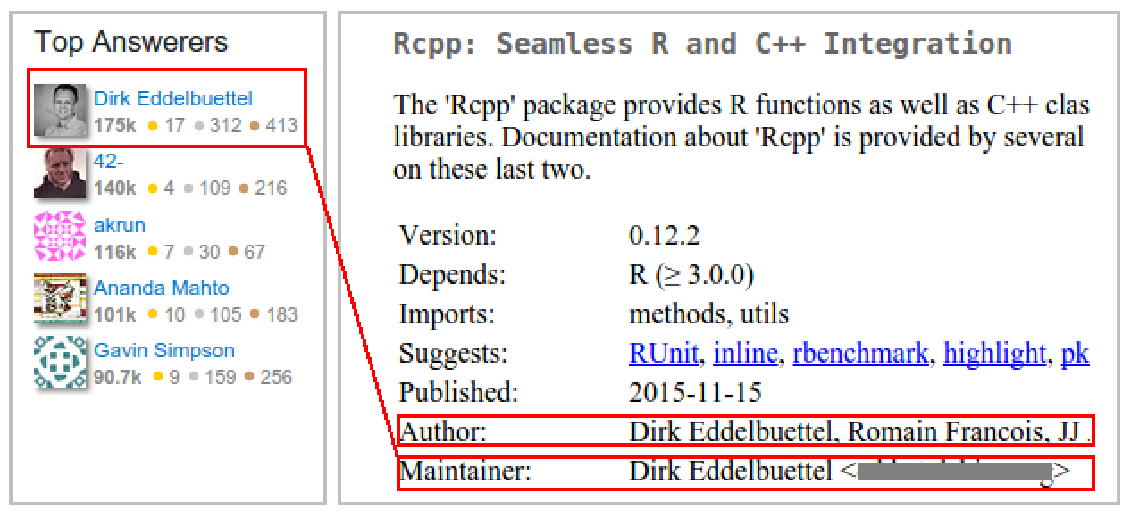
\includegraphics[width=\columnwidth]{Figures/CCchannel}
%        \caption{Example of how to reach developers of the \emph{rcpp} package. On the left, \SO, and on the right, the \emph{rcpp} webiste.}
%        \label{fig:CCchannel}
%    \end{figure}

%    Some channels are more suitable for certain \emph{type or format of questions}. 


\subsubsection{\recb}

    Throughout this study, we noticed that most of the harsh responses were given to users who did not learn the participation rules or had not learned the basic concept of R or statistics.
    For anybody using a channel, the community expects users to familiarize themselves with the channel in advance and learn the basics of the technology that they are discussing.

    % For instance, in the \RH's thread \textit{\href{http://goo.gl/Dc8gXw}{``Quantile''}} it is remarked the points of a guide that the user asking the question did not follow: \textit{``...Please read the Posting Guide. It asks that you not crosspost. If you post a followup to rhelp, then the reading of the Posting guide will tell you that much more in the way of detail about your setup was requested...''}.

%    Depending on the channel, the amount of guide lines and posting guides available might differ. 
    \SO provides user guides\footnote{\url{http://stackoverflow.com/help}} for each of the main features of the channel, such as badges, questions,
    answers, flags, comments, and the reputation system. While, the \RH mailing list only has general instructions\footnote{\url{https://www.r-project.org/mail.html\#instructions}} and a guide about posting on the channel\footnote{\url{https://www.r-project.org/posting-guide.html}}.

We also discovered that the R community has developed resources to improve the quality of participation on the communication channels.
%    Moreover, depending on the purposes of the \channels, there might exist community-developed guide that should be read before participating in the channel.
    For example, the post on \SO \textit{``How to make a great R reproducible example?''}\footnote{\href{http://stackoverflow.com/questions/5963269/how-to-make-a-great-r-reproducible-example}{http://stackoverflow.com/questions/5963269/how-to-make-a-great-r-reproducible-example}} provides tips and tricks for creating a reproducible example using the R language.
    Another example is the document \emph{How to write a reproducible
      example}\footnote{\url{http://adv-r.had.co.nz/Reproducibility.html}}, which provides tips for posting a reproducible R code example to mailing lists: \textit{``...Before putting all of your code in an email, consider putting it on \url{http://gist.github.com/}{[GitHub Gist app]}. It will give your code nice syntax highlighting, and you don't have to worry about anything getting mangled by the email system...''}

    Finally, there are manuals like \textit{``An Introduction to R''}, and the FAQ Webpages for R that are available to the public---most of the time, free of charge---and from which any user can learn the basics of R.
    For example, the R community provides a compendium of PDF documents for new users of different languages\footnote{The R manuals are available at \url{https://cran.r-project.org/}}.
    In \SO, supported technologies are provisioned with Webpages and links to free and paid materials\footnote{Materials available at \url{http://stackoverflow.com/tags/r/info}}.
    %Members are able to reference these materials when needed, e.g., \textit{``...You may want to acquaint yourself with the 'An Introduction to R' manual that came with your R installation to learn more about indexing.''}



\subsubsection{\recc}

    In spite of reading the documentation, a user may fail to address the channel appropriately.
    The community may feel that the question asked, the information provided, or something else entirely is not in compliance with the expectations and rules of the channel.
    In such cases, one should describe the documentation read, the attempts made, and the goal(s) they want to achieve.
    This would avoid answers like \textit{``read the manual''} or \textit{``read the posting guide''}. %, as well as helping the participants to help.
    For example, in the thread \textit{``lme4 GLMM''}\footnote{\url{https://goo.gl/Gbek3R}}, the user explicitly acknowledged the repeated question and explained the rationale for doing so: \textit{``I'm very sorry for my repeated question, which I asked 2 weeks ago, namely: I'm interested in possibly simple random-part specification in the call...''}.


\subsubsection{\recd}

    A common practice to answer or ask questions is to provide links for documentation, examples, source code, or other resources.
    As links point to online resources that might not exist in the future, it is important to include the key points of the resource within the question or answer.
    For instance, when a question or answer contains information in an external file hosting service like Dropbox or Google Drive, the owner of the service account can remove or break the link at any moment, leaving the message incomplete or impossible to reproduce. %An example can be seen in the thread\textit{\href{http://goo.gl/5nanFU}: {``Is it possible to create a 3D contour plot without continuous data in R?''}}.
    P33 suggested that \textit{``Questions should be self-contained as much as possible. Exceptions: recognizable links such as CRAN, R documentation, etc.''}.

    Based on our observations, we provide the following set of recommendations for using third-party resources within links.

    \begin{description}[itemsep=3pt, topsep=2pt, leftmargin=1em, parsep=0pt]
        \item[Use well-maintained Websites] that are expected to be available in the future, such as Wikipedia and the official documentation in CRAN.
        For example, %in the \SO thread \textit{``calculating convolution of multinomial distribution''},
        a user on \SO posted: \textit{``I'm doing a simulation where I need to calculate a \href{https://en.wikipedia.org/wiki/Convolution_of_probability_distributions}{[Wikipedia link] convolution} of
          \href{https://en.wikipedia.org/wiki/Multinomial_distribution}{[Wikipedia link] multinomial distributions}...''}.

        \item[Use resources that support or expand the message] to further clarify the message for those who might need it. For instance, a thread on \SO titled \textit{``How do I save all the draws from a MCMC posterior distribution to a file in R''} states \textit{``...You should be able to open a text connection using ?file \href{http://stat.ethz.ch/R-manual/R-devel/library/base/html/connections.html}{[more information]} with the open argument set to write...''}.

        \item[What to do when material relevant to the message is too big.] It is not always practical to include all the related information in a message. In this
          case, a link might be a better alternative, such as referencing videos or documents as links rather than including them as attachments.
        For example, in the \RH thread \textit{``Using FUNCTION to create usable objects''}, a user linked to a PDF rather than quoting it: \textit{``I suspect you are trying to find your way
          into Circle 6 of `The R Inferno' but haven't yet got in. \href{http://www.burns-stat.com/pages/Tutor/R\_inferno.pdf}{[link to PDF of R Inferno]}''}.
    \end{description}

\subsubsection{\rece}
\label{sec:userbeh}

It is obvious that users help others by answering questions. However, while analyzing questions and answers, we identified positive user behaviours that
we believe are worth mentioning.  These behaviours provide evidence of an altruistic way of thinking and the strong commitment that users have towards building knowledge in their community.

\begin{description}[itemsep=2pt, topsep=0pt, leftmargin=1em, parsep=0pt]
\item[I answered my own question:] Some questions are answered by the user that asked the question. They posted back to the channel to document their solution and help others: \textit{``Just for the records (and if anyone ever wants to find the `solution'), I solved my own problem.''}\footnote{\url{https://goo.gl/r3z0DX}}. 
 
\item[I did it for you:] When answering, authors provide source code to help others: \textit{``I coded up the algorithm from the Cameron and Turner paper. Dunno if it gives exactly the same results as my (Splus?) code from lo these many years ago...''}\footnote{\url{http://goo.gl/GXWGG3}}.

\item[Updated or continued years later:] Some questions are answered months or years later.
For example, a user on \SO modified an answer to provide a more updated version of the source code\footnote{\url{http://goo.gl/k6ZARR}}, and a {question asked on the \RH mailing list in 2012 was continued two years later}\footnote{\url{http://goo.gl/kgSHZv}}.

\item[Ideas to improve the channel:] This behaviour is specific to the \RH mailing list. Sometimes users suggest modifications or new features to improve the channel. For example, a {user proposed to create a package repository that can be accessible through a public wiki or version control interface}\footnote{\url{http://goo.gl/p0IunD}}.
\end{description}

% \dmg{I would remove the two following bullets:}

%     We also identified 2 behaviours that might result in a negative response from the community:
%     \begin{packed_enum}
%         \item \textbf{Cross-posting:} The user posts the same question in both channels at the same time.
%         For instance: \textit{\href{http://goo.gl/ENKrVK}{``-1 for cross posting to \RH – [user name]''}}.
% \dmg{This needs an example of a bad response, not just a crossposting, since this example does not show why users dislike it}
% \dmg{This next one sounds repetitive... it is already above in learn to use the chnanel}
%         \item \textbf{Posting guidelines violation:} The user behaves in a way that it becomes apparent that they did not read the posting guidelines.
%         For instance, a user asked a question that seems to be the opposite of what the posting guide recommend, and someone answered: \textit{\href{http://goo.gl/FUm1HC}{``...If you read the Posting Guide I think you will find precisely the opposite expectation explicitly presented. Using my "cheeky code" would only be part of the recommended actions to take before posting if you follow the recommendations of the "Do your homework before posting:"...''}}.
%     \end{packed_enum}

%\dmg{This section needs a way to finish}


\subsection{Threats to Validity}
\label{cha:threats}
Here we examine and discuss threats to the validity of our approach~\cite{Runeson2012}.
%\dmg{This is a section that can be shorten as needed in case of space issues... but first we need to finish the sections before }

%\remarks{Consider making the data available online.}
\begin{description}[itemsep=3pt, topsep=2pt, leftmargin=1em, parsep=0pt]

\item[Construct validity:] to reach the emerging themes, we rely on subjective human judgment during the data coding phase. Researchers had to decide if a message falls within a specific coding category. To alleviate this issue, two researchers coded the qualitative data as part of the analysis process. We applied the Cohen Kappa coefficient on categories that were not mutually exclusive, whose purpose was to trigger discussion between coders. We set a threshold of 0.8 as the minimum to obtain agreeable results, which is higher than the 0.6 suggested in the literature~\cite{Landis1977}.
%To minimize this threat, we used multiple data sources to triangulate our findings (survey, documentation, and messages from two different \channels), we randomly selected data, and two researchers performed the data coding.  

\item[Internal validity:] \SO's data is structured while \RH consists of unstructured data. As a result some of the mapping between both channels was straightforward (e.g., a follow-up to a reply is a comment to that question), while in other cases it wasn't as obvious (e.g., identifying some emails as questions). To reduce risk of bias when mapping the messages between both channels, two researchers performed the mapping.  


% in order to compare the emails to the \SO discussions we had to map the types of messages from one channel to the
% other. The \RH mailing list is unstructured emails that are connected between each other when they belong to the same thread. In contrast, \SO has a rich
% data type (questions, answers, comments, flags, etc.). Some of this mapping is automatic: a reply is a response to the original question, a follow-up to a reply
% is a comment to that question. Other had to be done by hand, this includes identifying some emails as containing a question, or a being a ``flag''.
% Also, \SO is newer than \RH, and for that reason we only used messages from \RH that were created after \SO was created.
% Two researchers performed this mapping to reduce any bias that it might have  introduced.

% Additionally, our understanding of that data and the observations we made played a big role in the mapping exercise, and it is subject to research bias.  To
% minimized the bias, two researches performed the mapping.

\item[External validity:] our case study is exploratory in nature and we purposefully aimed to study the R community. Many R users are likely to be \textit{casual developers} with limited or non-existent programming experience, and with backgrounds that vary from biologists to statisticians. Thus our findings may not apply to other developer communities. However, since \SO and mailing lists are widely used by other communities, we believe that our findings may be extended to these communities as well~\cite{Squire2015a}. We do not claim the generalazability of our findings to other communication channels (e.g., Slack, GitHub), and further research is required to examine how knowledge is shared on other channels used by developers.

% This type of case study cannot be assumed to be generalizable until further evaluations have been conducted~\cite{Yin2009}.
%     Hence, the findings of this research should be tested in other communities and with other channels to see if they apply to these other contexts.
% Another aspect to consider is that the R-community might not be composed of traditional programmers.
%     The R programming language is used to solve statistical problems, where the product is the statistical analysis or graphs it creates. The scripts written in
%     R are not the product, but the means to a product.
%     Also, many R language users are likely to be \textit{casual developers} with limited or non-existent programming experience, with backgrounds that vary from
%     biologists to statisticians. As a consequence, this study might not represent the knowledge that a software developer community shares. 
\end{description}

%%% Local Variables:
%%% mode: latex
%%% TeX-master: "knowledge-curation.tex"
%%% End:
